\documentclass[border=2pt]{standalone}
\usepackage{tikz}
\usetikzlibrary{positioning,arrows.meta,shapes.geometric}
\begin{document}
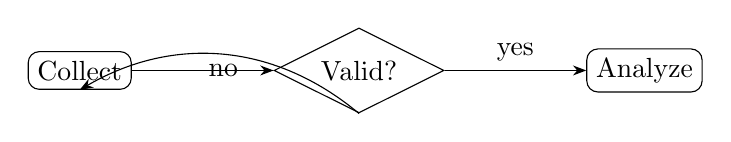
\begin{tikzpicture}[node distance=12mm and 18mm]
  \node[draw,rounded corners] (a) {Collect};
  \node[draw,diamond,aspect=2,right=of a] (b) {Valid?};
  \node[draw,rounded corners,right=of b] (c) {Analyze};
  \draw[-{Stealth}] (a)--(b); \draw[-{Stealth}] (b)--node[above]{yes}(c);
  \draw[-{Stealth},bend right=35] (b.south) to node[below]{no} (a.south);
\end{tikzpicture}
\end{document}
